% !TEX root = main.tex

\section{E-R模型} % Chap 7
在设计一个数据库模式时,要避免以下两个缺陷:
\begin{itemize}
	\item 冗余:可能导致不同关系表中的信息没有及时更新
	\item 不完整:只有对应开课的实体而没有对应课程的实体
\end{itemize}

\subsection{实体-关系模型}
\begin{definition}[实体]
实体是现实世界中可区别于所有其他对象的一个事物或对象。
每个实体有一组性质/属性(attribute),其中一些性质的值可以唯一标识一个实体。
实体集则是相同类型具有相同属性或性质的一个实体集合。
实体集是一个抽象概念,而实体集的外延(extension)则是指属于实体集实体的实际集合。
\end{definition}

大学中实际教师的集合构成了实体集instructor的外延。
实体集不必互不相交,如定义大学里所有人的实体集(person)。
一个person实体可以是instructior实体,可以是student实体,可以既是instructor实体又是student实体,也可以都不是。

\begin{definition}[联系]
联系(relationship)是指多个实体间的相互关联。
联系集是相同类型联系的集合。
\[\{(e_1,e_2,\ldots,e_n)\}\mid e_1\in E_1, e_2\in E_2, \ldots, e_n\in E_n\]
联系也可以具有\underline{描述性属性}(如下右图)。
\begin{figure}[H]
\centering
\begin{tabular}{cc}
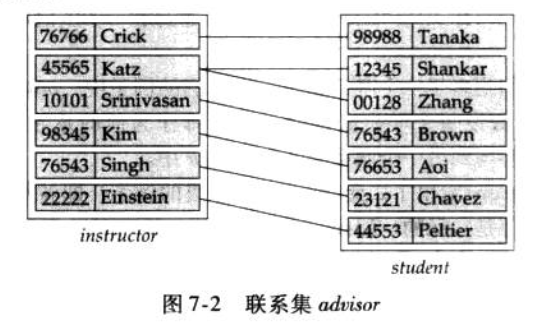
\includegraphics[width=0.5\linewidth]{fig/relationship_set.png}
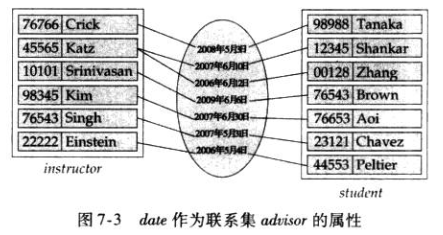
\includegraphics[width=0.5\linewidth]{fig/relationship_set(description).png}
\end{tabular}
\end{figure}
实体集之间的关联称为参与(participation),若$E$中每个实体都参与到联系集$R$中的至少一个联系中,则称参与是全部的(total)的,否则是部分的(partial)。
E-R模式中的联系实例则为具体命名实体间的关联。
实体在联系中扮演的功能称为实体的角色(role)。
参与联系集的实体集数目称为联系集的度(degree),二元联系集的度为2,三元联系集度为3。
\end{definition}

\begin{definition}[属性]
每个属性都有一个可取值的集合,称为该属性的域(domain),或值集(value set)。
属性可以分为简单和复合(composite)属性,复合属性可以再划分为更小的部分,如名字分为名和姓。
也可能是单值或多值属性,比如老师可以有多个电话号码,这是多值属性。
还有派生(derived)属性,可以通过其他属性计算得出。
\end{definition}
通常如果一个属性在两个实体集中出现,且这两个实体集存在关联,则该属性是冗余的,需要被移除。

\begin{definition}[映射基数(mapping cardinality)/基数比率]
一个实体通过一个联系集能关联的实体个数,包括了一对一、一对多(many)、多对一、多对多这几种情况。
one代表至多一个,many代表零个或多个。
\begin{figure}[H]
\centering
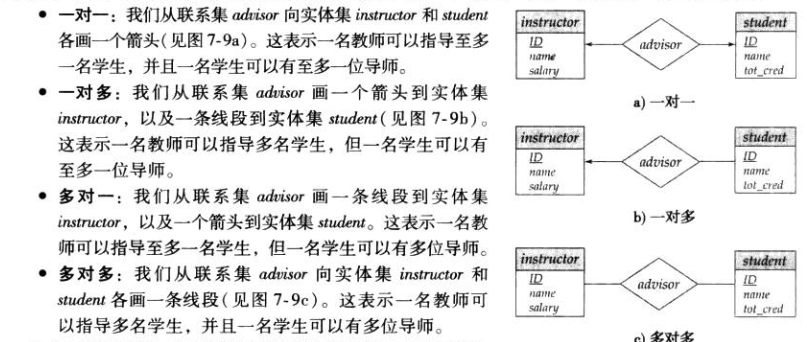
\includegraphics[width=\linewidth]{fig/mapping_radix.png}
\end{figure}
\end{definition}
也可以采用更为复杂的映射基数$l..h$的形式表示,其中$l$表示最小映射基数,$h$为最大映射基数。
最小值为$1$代表这个实体集在该联系集中全部参与,最大值为$1$表示这个实体至多参与一个联系,最大值为$*$则没有限制。

\begin{definition}[角色]
联系集产生自环,如course有前置课程prereq\_id
\end{definition}
\begin{definition}[强弱实体集]
没有足够属性形成主码的实体集称为弱实体集,有主码的实体集则称为强实体集。
弱实体集必须与另一个称作标识(identifying)或\textbf{属主(owner)实体集}的实体集关联才有意义。
弱实体集的\textbf{分辨符}(discriminator)/部分码是使得能够区分弱实体集中实体的方法,用虚下划线标明。
\end{definition}

比如section实体由课程编号、学期、学年及开课编号唯一标识。
假定在实体集section和course之间创建了联系集sec\_course,由于section中已有属性course\_id,故在联系集中存在冗余,要将course\_id删除,但这会导致section没有主码。
因而将联系sec\_course视为特殊的联系,它给唯一标识section实体提供额外信息,即course\_id。

E-R图,菱形代表联系,双横线代表全部参与,双框代表弱实体集。
\begin{figure}[H]
\centering
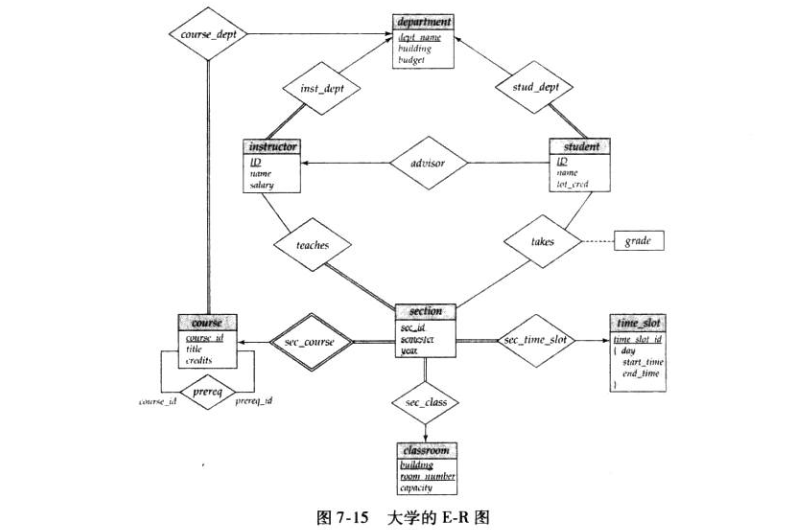
\includegraphics[width=0.6\linewidth]{fig/university_E-R.png}
\end{figure}
\begin{figure}[H]
\centering
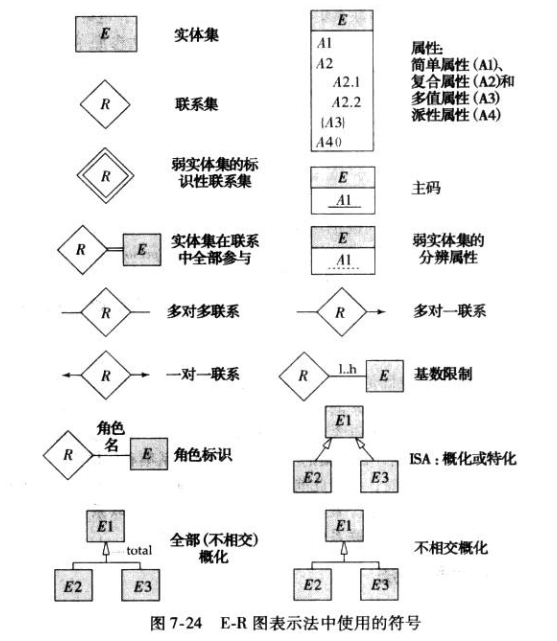
\includegraphics[width=0.5\linewidth]{fig/E-R-figure.png}
\end{figure}

一个常见的错误是将一个实体集的主码作为另一个实体集的属性(关系被隐藏了),而不是使用联系。

\subsection{转化为关系模式}
\begin{itemize}
	\item 简单属性强实体集直接转关系模式,如
	\[student(\underline{ID},name,tot\_cred)\]
	\item 复杂属性强实体集展平后转关系模式,如名字含first\_name和last\_name,那就一起放入关系模式
	\item 弱实体集由\textemph{其依赖的强实体集主码与自身}组成,主码为强实体集主码与弱实体集分辨符,且要在关系$A$上建立外码约束
	\item 联系集:\textemph{所有参与该联系的实体集的主码的并集}构成属性集合(弱实体集则要带上其依赖的强实体集主码),依据下列规则选择主码:
	\begin{center}
	\begin{tabular}{|c|c|c|}\hline
		A & B & 主码\\\hline
		多 & 多 & A+B\\\hline
		多 & 一 & A\\\hline
		一 & 多 & B\\\hline
		一 & 一 & A/B\\\hline
	\end{tabular}
	\end{center}
	对于每个与联系集$R$相关的实体集$E_i$,建立关系模式$R$上的外码约束,$R$中来自$E_i$主码属性的那些属性参照表示关系模式$E_i$的主码。
	如大学关系模式中,advisor为多对一联系,则建立关系模式
	\[advisor(\underline{s\_ID},i\_ID)\]
\end{itemize}

通常,连接弱实体集与其依赖的强实体集的联系集的模式是冗余的,在基于E-R图的关系数据库设计中不必给出。

当出现以下两种情况时,需要对关系模式进行合并:
\begin{itemize}
	\item 实体集$A$到实体集$B$是一个多对一的联系集$AB$,且$A$的参与是全部的,则将$A$和$AB$合并,如inst\_dept可以和instructor合并为
	\[instructor(ID,name,dept\_name,salary)\]
	\item 一对一则联系集可以跟参与联系的任一个实体集模式进行合并
\end{itemize}

\subsection{扩展的E-R属性}
\begin{definition}[特化和泛化]
在实体集内部进行分组的过程称为特化(specialization),如将实体集person划分为employee和student。
概化(generalization)则是自底向上的反过程。
高层与低层实体集也可被分别称为超类和子类,同样有继承(inheritance)的特性。
如果一个实体集作为低层实体集参与到多个联系中,则称这个实体集具有多继承,且产生的结构称为格(lattice)。
\end{definition}

\begin{definition}[聚集]
聚集是一种抽象,其中联系集和跟它们相关的实体集一起被看作高层实体集,并且可以参与联系。
\end{definition}